\documentclass[xcolor={x11names,svgnames}]{beamer}
\setbeamerfont{note page}{size=\tiny} % default = small 

%\includeonlyframes{roofline_intro}

\usecolortheme{rose}
\setbeamertemplate{footline}{}
\setbeamertemplate{navigation symbols}{\footnotesize\insertframenumber}
  
\usepackage{amsmath, amssymb, amsthm}

\usepackage[utf8]{inputenc}
\usepackage[francais]{babel}
\usepackage[T1]{fontenc}
\usepackage[normalem]{ulem}   
\usepackage{mdframed}
\usepackage{multirow}

\usepackage{minted}
%\setminted{fontsize=\scriptsize}
\newcommand{\bigO}[1]{\ensuremath{\mathcal{O}\left( #1 \right)} }

\usepackage{tikz}
\usetikzlibrary{calc}
\usetikzlibrary{decorations}
\usetikzlibrary{positioning}
\usetikzlibrary{decorations.pathmorphing}
\usetikzlibrary{decorations.pathreplacing}
\usetikzlibrary{shapes.multipart}
\usetikzlibrary{math}

\usepackage{fontspec}

\setsansfont{PalatinoSansLTPro}[
   Path = /home/charles/charles_work/fonts/PalatinoSans/, 
   Extension      = .otf,
   UprightFont    = *-Regular,
   BoldFont= *-Bold ,
   ItalicFont = *-Italic,
   BoldItalicFont = *-BoldIta
]

\newcommand{\blue}[1]{{\color{Blue}#1}}
%\newcommand{\green}[1]{{\color{LimeGreen}#1}}
\newcommand{\red}[1]{{\color{red}#1}}
\newcommand{\tikzmat}[2] {
\draw[thick] let \p1 = (#1 |- #2),
                 \p2 = (#2 |- #1) in
   ($ (#1) + (0.05,-0.1) $) -- ++(-0.15, 0)  -- ($ (\p1) + (-0.1,0.1) $) -- ++(0.15,0)
   ($ (\p2) + (-0.05,-0.1) $) -- ++(0.15, 0) -- ($ (#2) + (0.1,0.1) $) -- ++(-0.15,0);
}


\author[C.~Bouillaguet]{Charles Bouillaguet \newline
  {\small \texttt{charles.bouillaguet@lip6.fr}}}

\title{Cours 9 : puissance de crête, équilibrage, intensité opérationnelle, etc.}


\begin{document}

\begin{frame}[label=title]
    \titlepage
  \end{frame}
  
%%%%%%%%%%%%%%%%%

\begin{frame}
  \frametitle{Jeu de rôle}
  \framesubtitle{Vous êtes le CNRS et vous venez de vous faire livrer}
  \centering
  \begin{columns}
    \begin{column}{4.75cm}
      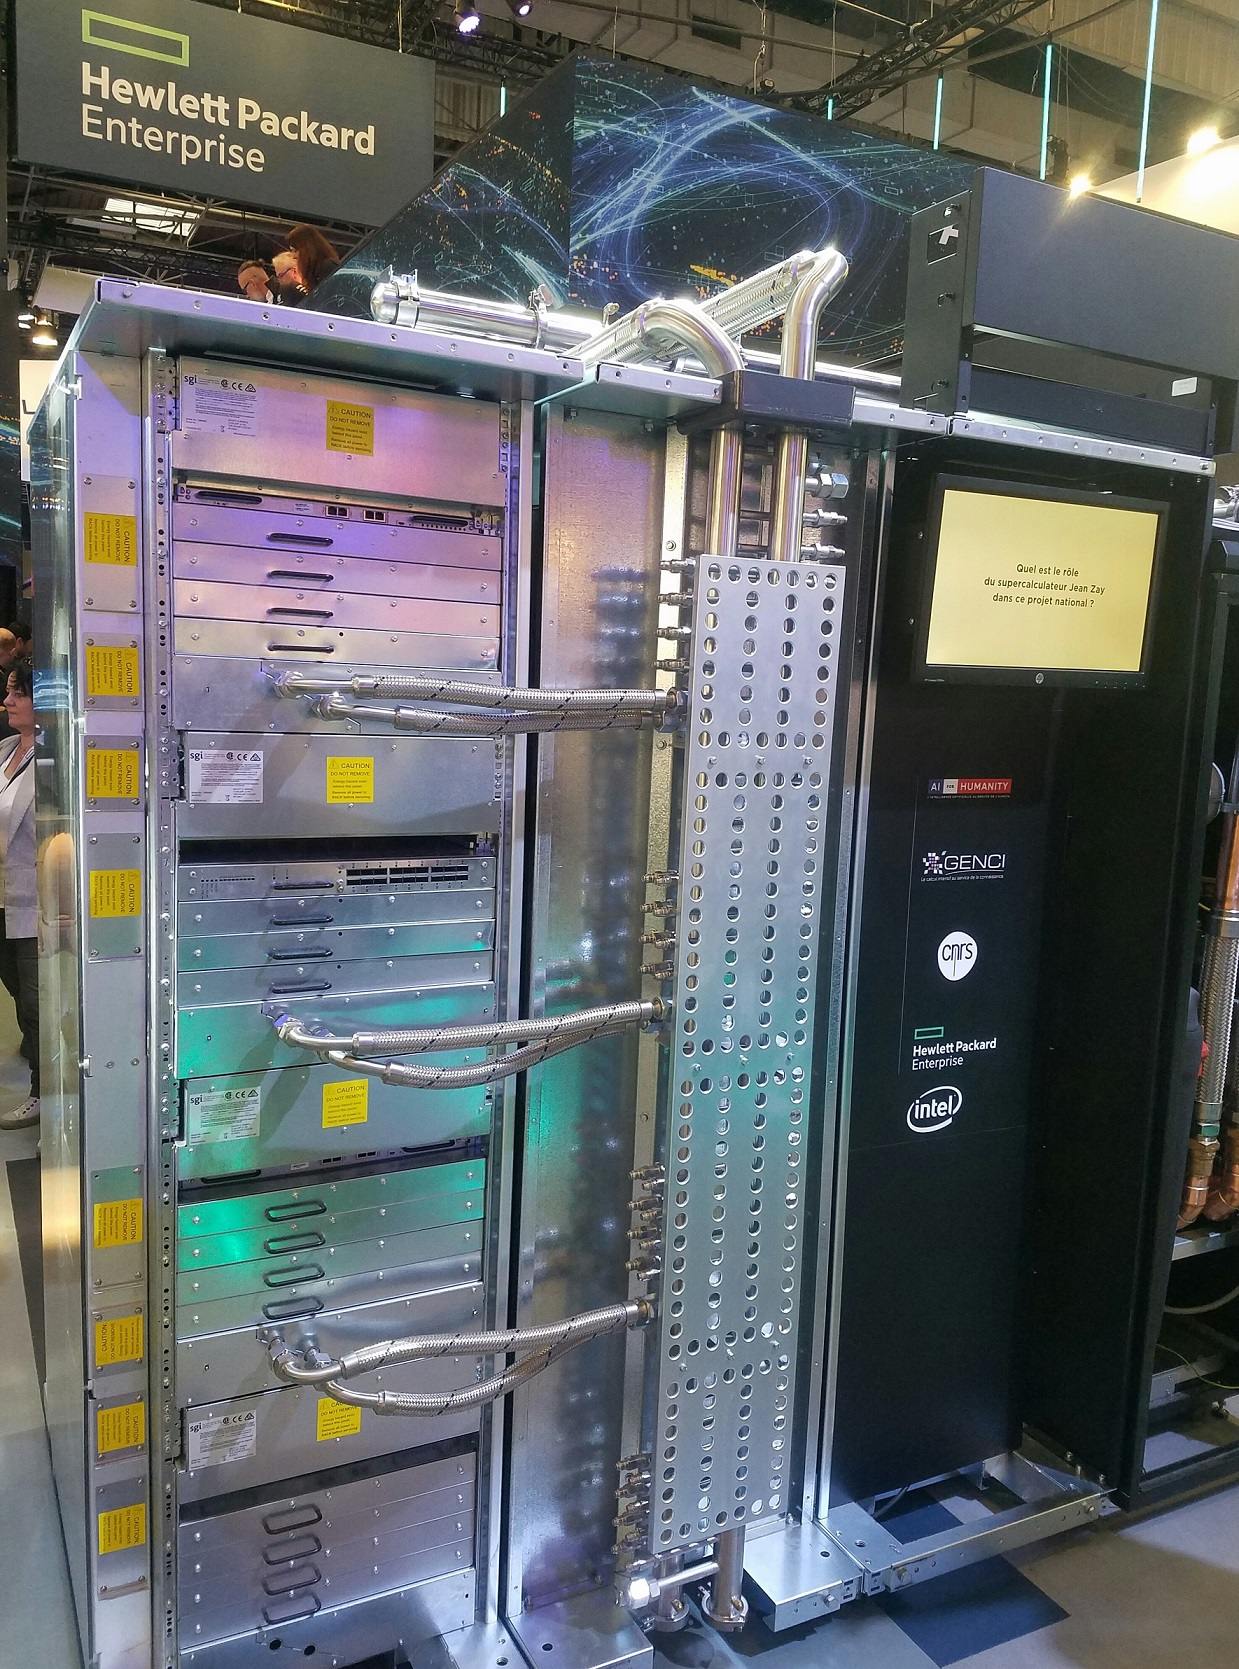
\includegraphics[height=7cm]{jean-zay}
    \end{column}
    \begin{column}{5.5cm}
      \small
      \begin{itemize}
      \item 1528 noeuds
      \item 2 $\times$ Xeon Gold 6248 (\og Cascade Lake\fg{})
      \item 20 coeurs @ 2.5 Ghz
      \item 192 Go RAM/noeud
      \item Omnipath 100Gbit/s
      \end{itemize}

      \begin{block}{Question légitime}
        À quel point ça va aller plus vite que le précédent ?
      \end{block}
    \end{column}
  \end{columns}
\end{frame}

%%%%%%%%%%%%%%%%%%%

\begin{frame}
  \frametitle{Puissance de crête}

  \begin{block}{Définition}
    Nombre maximal de FLOPS que le hardware peut (en théorie) effectuer.
  \end{block}

  \begin{itemize}
  \item Noeuds
  \item SMP ?
  \item Fréquence CPU
  \item Coeurs
  \item Unités SIMD
  \item Parallélisme d'instruction
  \item Fused Multiply-Add
  \end{itemize}
  
\end{frame}

%%%%%%%%%%%%%%%%

\begin{frame}
  \frametitle{Cas facile}
  \framesubtitle{Turing}

  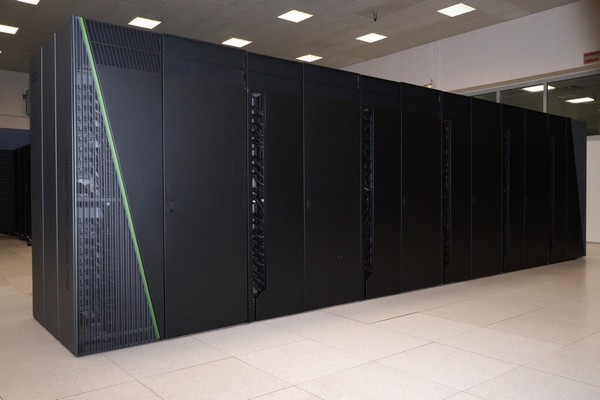
\includegraphics[width=\textwidth]{turing}
\end{frame}

\begin{frame}
  \frametitle{Cas facile}
  \framesubtitle{Turing}

  \begin{itemize}
  \item Noeuds : 6144
  \item CPU : PowerPC A2 @ 1.6Ghz
  \item Coeurs : 16
  \item Unités SIMD : 256-bits (4 doubles)
  \item Fused Multiply-Add : oui
  \item 1 instruction/cycle maximum
  \end{itemize}

  \begin{alertblock}{Résultat}
    $6144 \times 1.6e9 \times 16 \times 4 \times 2 = 1144$ TeraFLOPS
  \end{alertblock}
\end{frame}

%%%%%%%%%%%%%%%%%%%

\begin{frame}
  \frametitle{Cas dur}
  \framesubtitle{Jean-Zay}

  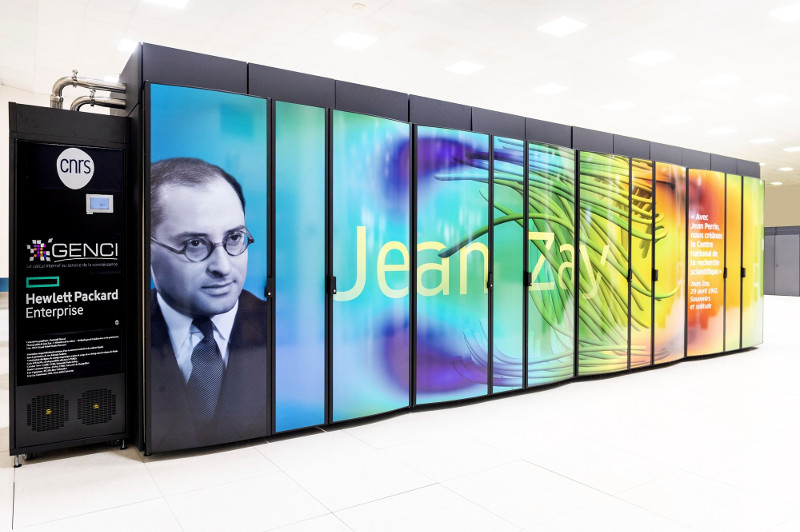
\includegraphics[width=\textwidth]{jean-zay-bis}
\end{frame}

\begin{frame}
  \frametitle{Cas dur}
  \framesubtitle{Jean-Zay}

  \begin{itemize}
  \item Noeuds : 1528
  \item CPU Xeon Gold 6248 @ \alert{[ça dépend]} GHz
  \item Coeurs : 20 (2 CPU / noeud)
  \item Unités SIMD : 512-bits (8 doubles)
  \item Fused Multiply-Add : oui
  \item instruction/cycle maximum : \alert{2 FMA}
    \begin{itemize}
    \item Certains Xeon : 1 seul
    \item D'autres Xeon : 2
    \end{itemize}
  \end{itemize}
\end{frame}

%%%%%%%%%%%%%%%%

\begin{frame}
  \frametitle{CPU Frequency Scaling}
  \framesubtitle{Problème d'enveloppe thermique}
  
  \begin{block}{La fréquence d'un coeur dépend}
  \begin{itemize}
  \item Du type d'instruction exécuté
  \item De ce que font les autres coeurs
  \item De la qualité du composant matériel
  \end{itemize}
\end{block}

\bigskip

Pour les Intel Xeon Gold 6248 :

\medskip

\centering
  \small
\begin{tabular}{|c|c||c|c|c|c|c|c|c|c|}
  \hline
  \multirow{2}{*}{Mode}   & \multirow{2}{*}{Base} & \multicolumn{6}{c|}{Turbo avec $x$ coeurs actifs} \\
%  \cline{3-23}
  & &             1-2 & 3-4 & 5-8 & 9-12 & 13-16 & 17-20 \\
  \hline\hline
  normal & 2.5	& 3.9 & 3.7 & 3.6 & 3.6 & 3.4 & 3.2 \\
  \hline
  AVX2	 & 1.9	& 3.8 & 3.6 & 3.5 & 3.4 & 3.0 & 2.8 \\
  \hline
  AVX512 & 1.6	& 3.8 & 3.6 & 3.5 & 3.0 & 2.7 & 2.5 \\
  \hline
\end{tabular}

\begin{alertblock}{Conclusion}
  \centering
  $\text{SSE } \xrightarrow{\times 3} \text{ AVX-2 } \xrightarrow{\times 1.7} \text{ AVX-512}$
\end{alertblock}

\end{frame}

%%%%%%%%%%%%

\begin{frame}
  \frametitle{Intensité Opérationnelle}

  \begin{block}{Rappel}
    On cherche à prévoir/comprendre les performances d'une application sur une machine donnée.
  \end{block}

  \begin{exampleblock}{Définition}
    L'\alert{intensité opérationnelle} d'un algorithme est le nombre
    d'opérations arithmétiques effectuées par octet transféré depuis la RAM.
  \end{exampleblock}
  
  \[
    IO = \dfrac{\text{FLOP}}{\text{Octets }\leftrightarrow\text{ RAM}}
  \]

  (see also: intensité arithmétique)
\end{frame}

%%%%%%%%%%%%%%%%%%%%%%%%%%%%%%%%%%%%%%%%%%%%%%%%%%%%%%%%%%%%%%%%%%%%%%%%%%%%%%

\begin{frame}[label=roofline_intro]
  \frametitle{Diagramme \emph{roofline} --- 1 coeur}
  \framesubtitle{Intérêt :     $\text{[FLOPS]} \leq \max \bigl( [\text{peak FLOPS}],  [IO] \times [\text{peak RAM BW}]\bigr)$}
    
  \begin{tikzpicture}[scale=0.8, font=\scriptsize]
    % outer box
    \draw[thick] (0, 0) rectangle +(12, 8);

    % help lines
    \foreach \i in {1, ..., 11}
    \draw[gray, semitransparent, densely dashed] (\i, 0) -- +(0, 8);

    \foreach \j in {1, ..., 7}
    \draw[gray, semitransparent, densely dashed] (0, \j) -- +(12, 0);

    % left labels
    \foreach \j / \lab in {0 / 1, 1 / 2, 2 / 4, 3 / 8, 4 / 16, 5 / 32, 6 / 64, 7 / 128, 8 / 256}
    \draw[] (0, \j) -- +(-0.1, 0) node[anchor=east,] {\lab};

    % left axis label
    \node[rotate=90, anchor=south] at (-1, 4) {Attainable GFLOP/s};

    % bottom labels
    \foreach \i / \lab in {0 / $\frac{1}{64}$, 1 / $\frac{1}{32}$, 2 / $\frac{1}{16}$, 3 / $\frac{1}{8}$, 4 / $\frac{1}{4}$,
      5 / $\frac{1}{2}$, 6 / 1, 7 / 2, 8 / 3, 9 / 4, 10 / 8, 11 / 16, 12 / 32}
    \draw[] (\i, 0) -- +(0, -0.1) node[anchor=north] {\lab};

    % left axis label
    \node[anchor=north] at (5, -0.75) {FLOP / byte};

    \begin{scope}
    \path[clip] (0, 0) rectangle +(12, 8);


    % peak CPU GFLOPS
    \fill<1-3>[nearly transparent, blue] (0, 2.3) rectangle (12, 8);
    \draw<1-3>[ultra thick, blue] (0, 2.3) -- +(12, 0) node[anchor=south east,text=black] at (12, 2.3) {scalar};
    \draw<4->[ultra thick, blue, dashed, nearly transparent] (0, 2.3) -- +(12, 0);

    
    \fill<4>[nearly transparent, blue] (0, 3.9) rectangle (12, 8);
    \draw<4>[ultra thick, blue] (0, 3.9) -- +(12, 0) node[anchor=south east,text=black] at (12, 3.9) {AVX2};
    \draw<5->[ultra thick, blue, dashed, nearly transparent] (0, 3.9) -- +(12, 0);

    
    \fill<5>[nearly transparent, blue] (0, 4.7) rectangle (12, 8);
    \draw<5>[ultra thick, blue] (0, 4.7) -- +(12, 0) node[anchor=south east,text=black] at (12, 4.7) {AVX512};
    \draw<6->[ultra thick, blue, dashed, nearly transparent] (0, 4.7) -- +(12, 0);

    
    \fill<6>[nearly transparent, blue] (0, 5.7) rectangle (12, 8);
    \draw<6>[ultra thick, blue] (0, 5.7) -- +(12, 0) node[anchor=south east,text=black] at (12, 5.7) {+FMA};
    \draw<7->[ultra thick, blue, dashed, nearly transparent] (0, 5.7) -- +(12, 0);

    
    \fill<7->[nearly transparent, blue] (0, 6.7) rectangle (12, 8);
    \draw<7->[ultra thick, blue] (0, 6.7) -- +(12, 0) node[anchor=south east,text=black] at (12, 6.7) {+ILP};


    % peak DRAM bandwith    
    \fill<2>[nearly transparent, orange] (0, 0) -- (2.13, 0) -- (10.13, 8) -- (0, 8) -- cycle;
    % 4 - log2(15)                            5 + 8 - log2(15) 
    \draw<2>[ultra thick, orange] (2.13, 0) -- node[pos=0.1, above, sloped, black] {Peak DRAM BW} (10.13, 8);
    \draw<3->[ultra thick, orange, nearly transparent, dashed] (2.13, 0) -- (10.13, 8);

    % peak L1
    \fill<3-7>[nearly transparent, orange] (0, 0) -- (-1.022, 0) -- (6.977, 8) -- (0, 8) -- cycle;
    \draw<3-7>[ultra thick, orange] (-1.022, 0) -- node[pos=0.36, above, sloped, black] {Peak L1 BW} (6.977, 8);

    % peak L2
    \fill<8>[nearly transparent, orange] (0, 0) -- (0.0811, 0) -- (8.0811, 8) -- (0, 8) -- cycle;
    \draw<8>[ultra thick, orange] (0.0811, 0) -- node[pos=0.125, above, sloped, black] {Peak L2 BW} (8.0811, 8);
  \end{scope}
  
  \end{tikzpicture}
\end{frame}

%%%%%%%%%%%%%%%%%%%%%%%%%%%%%%%%%%%%%%%%%%%%%%%%%%%%%%%%%%%%%%%%%%%%%%%%%%%%%%%%%%%%%%

\begin{frame}[label=roofline_intro]
  \frametitle{Diagramme \emph{roofline} --- 1 coeur (résumé)}
  \framesubtitle{Intérêt :     $\text{[FLOPS]} \leq \max \bigl( [\text{peak FLOPS}],  [IO] \times [\text{peak RAM BW}]\bigr)$}
    
  \begin{tikzpicture}[scale=0.8, font=\scriptsize]
    % outer box
    \draw[thick] (0, 0) rectangle +(12, 8);

    % help lines
    \foreach \i in {1, ..., 11}
    \draw[gray, semitransparent, densely dashed] (\i, 0) -- +(0, 8);

    \foreach \j in {1, ..., 7}
    \draw[gray, semitransparent, densely dashed] (0, \j) -- +(12, 0);

    % left labels
    \foreach \j / \lab in {0 / 1, 1 / 2, 2 / 4, 3 / 8, 4 / 16, 5 / 32, 6 / 64, 7 / 128, 8 / 256}
    \draw[] (0, \j) -- +(-0.1, 0) node[anchor=east,] {\lab};

    % left axis label
    \node[rotate=90, anchor=south] at (-1, 4) {Attainable GFLOP/s};

    % bottom labels
    \foreach \i / \lab in {0 / $\frac{1}{64}$, 1 / $\frac{1}{32}$, 2 / $\frac{1}{16}$, 3 / $\frac{1}{8}$, 4 / $\frac{1}{4}$,
      5 / $\frac{1}{2}$, 6 / 1, 7 / 2, 8 / 3, 9 / 4, 10 / 8, 11 / 16, 12 / 32}
    \draw[] (\i, 0) -- +(0, -0.1) node[anchor=north] {\lab};

    % left axis label
    \node[anchor=north] at (5, -0.75) {FLOP / byte};

    \begin{scope}
    \path[clip] (0, 0) rectangle +(12, 8);

    % peak CPU GFLOPS
    \draw[ultra thick, blue] (0, 2.3) -- +(12, 0) node[anchor=south east,text=black] at (12, 2.3) {scalar};
    \draw[ultra thick, blue] (0, 3.9) -- +(12, 0) node[anchor=south east,text=black] at (12, 3.9) {AVX2};
    \draw[ultra thick, blue] (0, 4.7) -- +(12, 0) node[anchor=south east,text=black] at (12, 4.7) {AVX512};
    \draw[ultra thick, blue] (0, 5.7) -- +(12, 0) node[anchor=south east,text=black] at (12, 5.7) {+FMA};
    \draw[ultra thick, blue] (0, 6.7) -- +(12, 0) node[anchor=south east,text=black] at (12, 6.7) {+ILP};

    % peak DRAM bandwith    
    \draw[ultra thick, orange] (2.13, 0) -- node[pos=0.1, above, sloped, black] {Peak DRAM BW} (10.13, 8);
    \draw[ultra thick, orange] (-1.022, 0) -- node[pos=0.36, above, sloped, black] {Peak L1 BW} (6.977, 8);
    \draw[ultra thick, orange] (0.0811, 0) -- node[pos=0.125, above, sloped, black] {Peak L2 BW} (8.0811, 8);
  \end{scope}
  
  \end{tikzpicture}
\end{frame}

%%%%%%%%%%%%%%%%%%%%%%%%%%%%%%%%%%%%%%%%%%%%%%%%%%%%%%%%%%%%%%%%%%%%%%%%%%%%%%%%%%%%%%

\begin{frame}[label=roofline_intro]
  \frametitle{Diagramme \emph{roofline} --- 1 noeud entier}
    
  \begin{tikzpicture}[scale=0.8, font=\scriptsize]
    % outer box
    \draw[thick] (0, 0) rectangle +(12, 9);

    % help lines
    \foreach \i in {1, ..., 11}
    \draw[gray, semitransparent, densely dashed] (\i, 0) -- +(0, 9);

    \foreach \j in {1, ..., 8}
    \draw[gray, semitransparent, densely dashed] (0, \j) -- +(12, 0);

    % left labels
    \foreach \j / \lab in {0 / 1, 1 / 2, 2 / 4, 3 / 8, 4 / 16, 5 / 32, 6 / 64, 7 / 128, 8 / 256, 9 / 512}
    \draw[] (0, \j) -- +(-0.1, 0) node[anchor=east,] {\lab};

    % left axis label
    \node[rotate=90, anchor=south] at (-1, 4) {Attainable GFLOP/s};

    % bottom labels
    \foreach \i / \lab in {0 / $\frac{1}{64}$, 1 / $\frac{1}{32}$, 2 / $\frac{1}{16}$, 3 / $\frac{1}{8}$, 4 / $\frac{1}{4}$,
      5 / $\frac{1}{2}$, 6 / 1, 7 / 2, 8 / 3, 9 / 4, 10 / 8, 11 / 16, 12 / 32}
    \draw[] (\i, 0) -- +(0, -0.1) node[anchor=north] {\lab};

    % left axis label
    \node[anchor=north] at (5, -0.75) {FLOP / byte};

    \begin{scope}
    \path[clip] (0, 0) rectangle +(12, 9);


    % peak CPU GFLOPS
    \fill<1-2>[nearly transparent, blue] (0, 3.9) rectangle (12, 9);
    \draw<1-2>[ultra thick, blue] (0, 3.9) -- +(12, 0) node[anchor=south east,text=black] {1 core (AVX2)};
    \draw<3->[ultra thick, blue, dashed, nearly transparent] (0, 3.9) -- +(12, 0);
    
    \fill<3>[nearly transparent, blue] (0, 8.5) rectangle (12, 9);
    \draw<3>[ultra thick, blue] (0, 8.5) -- +(12, 0) node[anchor=north east,text=black] {32 cores (AVX2)};

    % 1 core
    \fill<2>[nearly transparent, orange] (0, 0) -- (-1.022, 0) -- (7.977, 9) -- (0, 9) -- cycle;
    \draw<2>[ultra thick, orange] (-1.022, 0) -- node[pos=0.25, above, sloped, black] {Peak L1 BW} (7.977, 9);
    \draw<3>[ultra thick, orange, dashed, nearly transparent] (-1.022, 0) -- (7.977, 9);

    \fill<2>[nearly transparent, orange] (0, 0) -- (2.13, 0) -- (11.13, 9) -- (0, 9) -- cycle;
    \draw<2>[ultra thick, orange] (2.13, 0) -- node[pos=0.1, above, sloped, black] {Peak DRAM BW} (11.13, 9);
    \draw<3->[ultra thick, orange, dashed, nearly transparent] (2.13, 0) -- (11.13, 9);

    % 32 cores
    \fill<3>[nearly transparent, orange] (0, 0) -- (-5.82, 0) -- (3.417, 9) -- (0, 9) -- cycle;
    \draw<3>[ultra thick, orange] (-5.82, 0) -- node[pos=0.8, above, sloped, black] {Peak L1 BW} (3.417, 9);

    \fill<3>[nearly transparent, orange] (0, 0) -- (-1.28, 0) -- (7.72, 9) -- (0, 9) -- cycle;
    \draw<3>[ultra thick, orange] (-1.28, 0) -- node[pos=0.3, above, sloped, black] {Peak DRAM BW} (7.72, 9);
  \end{scope}
  
  \end{tikzpicture}
\end{frame}


%%%%%%%%%%%%%%%%%%%%%%%%%%%%%%%%%%%%%%%%%%%%%%%%%%%%%%%%%%%%%%%%%%%%%%%%%%%%%%%%%%%%%%

\begin{frame}[fragile]
  \frametitle{Intensité Opérationnelle}
  \framesubtitle{Petits exemples}
  
  \begin{block}{Produit scalaire}
\begin{minted}{C}
double res = 0;
for (int j = 0; j < N; j++)
    res += A[i] * B[i];
\end{minted}
  \end{block}

  \pause

  \bigskip

  \[
    IO = 1 \text{FLOP / double} = 1/8
  \]  
\end{frame}

%%%%%%%%%%%%%%%%%%%%%%%%%

\begin{frame}[fragile]
  \frametitle{Intensité Opérationnelle}
  \framesubtitle{Petits exemples}
  
  \begin{block}{Produit matrice-vecteur}
\begin{minted}{C}
for (int i = 0; i < N; i++) {
    y[i] = 0.0;
    for (int j = 0; j < N; j++)
        y[i] += A[i*N + j] * x[j];
}
\end{minted}
  \end{block}

  \pause

  \bigskip

  \[
    IO = \begin{cases}
      \text{2 FLOP / double} = 1 / 4 & \text{ si $x$ tient en cache} \\
      \text{1 FLOP / double} = 1 / 8 & \text{ sinon}
    \end{cases}
  \]  
\end{frame}

%%%%%%%%%%%%%%%%%%%%%%%%

\begin{frame}[fragile]
  \frametitle{Intensité Opérationnelle}
  \framesubtitle{Petits exemples}
  
  \begin{block}{Produit matrice creuse-vecteur dense}
\begin{minted}{C}
for (int k = 0; i < NNZ; i++) {
    int i = Ai[k];
    int j = Aj[k];
    y[i] += Ax[k] * x[j];
  }
}
\end{minted}
  \end{block}

  \pause

  \[
    IO = \begin{cases}
      1 / 8  & \text{ si $x$ tient en cache} \\
      1 / 12 & \text{ sinon}
    \end{cases}
  \]  
\end{frame}

%%%%%%%%%%%%%%%%%%%%%%%%%

\begin{frame}[fragile]
  \frametitle{Améliorer l'intensité opérationnelle ?}

  \begin{itemize}
  \item En général, il faut changer les algos (\emph{blocking}...)
  \item Optimisation generique : \emph{loop fusion}.
  \end{itemize}

  \bigskip
  
  \begin{columns}[T]
    \begin{column}{0.5\textwidth}
\begin{minted}[fontsize=\scriptsize]{C}
/* Mauvais */
for (int i = 0; i < N; i++)
    A[i] += B[i] * C[i];
for (int i = 0; i < N; i++)
    D[i] += B[i] + E[i];
\end{minted}
    \end{column}
    \begin{column}{0.5\textwidth}
\begin{minted}[fontsize=\scriptsize]{C}
/* Meilleur */
for (int i = 0; i < N; i++) {
    double Bi = B[i];
    A[i] += Bi * C[i];
    D[i] += Bi + E[i];
}
\end{minted}
    \end{column}
  \end{columns}

  \begin{itemize}
  \item[$\rightarrow$] projet 
  \end{itemize}
\end{frame}

%%%%%%%%%%%%%%%%%%%%%%%%%%%%%%%%%%%%%%%%%%%%%%%%%%%%%%%%%%%%%%%%%%%

\begin{frame}[fragile, label=blocking]
  \frametitle{Améliorer l'intensité opérationnelle ?}

  \begin{itemize}
  \item En général, il faut changer les algos (\alert{\emph{blocking}}...)
  \end{itemize}

  \begin{center}
    \begin{tikzpicture}
    \draw[thick, fill=LimeGreen] (-1, 0) rectangle +(0.25, 4);
    \draw[thick, fill=red] (4.75, 0) rectangle +(0.25, 4);
    \draw[thick, fill=cyan] (0, 0) rectangle (4, 4);
    \node at (-0.375, 2) {=};
    \node at (4.375, 2) {$\times$};
    \foreach \i in {1, 2, 3} {
      \draw (\i, 0) -- +(0, 4);
      \draw (0, \i) -- +(4, 0);
      \draw (-1, \i) -- +(0.25, 0);
      \draw (4.75, \i) -- +(0.25, 0);
    }
  \end{tikzpicture}
\end{center}

\begin{itemize}
\item Charger un bout de $x$ en cache
\item Charger un bout de $y$ en cache (y est déjà ?)
\item Faire le produit avec le bloc de $A$ qui correspond
  \begin{itemize}
  \item $A$ lu depuis la RAM
  \end{itemize}
\item Recommencer avec le bloc suivant
\end{itemize}
\end{frame}

%%%%%%%%%%%%%%%%%%%%%%%%%%%%%%%%%%%%%%%%%%%%%%%%%%%%%%%%%%%%%%%%%%%%
              
\begin{frame}[fragile]
  \frametitle{Améliorer l'intensité opérationnelle ?}

  \begin{itemize}
  \item En général, il faut changer les algos...
  \item ... ou les structures de données
  \end{itemize}

  \bigskip

  \begin{block}{Produit matrice creuse-vecteur dense}
\begin{minted}{C}
for (int k = 0; i < NNZ; i++) {
    int i = Ai[k];
    int j = Aj[k];
    y[i] += Ax[k] * x[j];
  }
}
\end{minted}
\begin{itemize}
\item Triplets triés par \texttt{Ai[...]} croissant 
\item[$\Rightarrow$] lit (souvent) le même $i$ que l'itération précédente 

  \pause

\item[$\leadsto$] \alert{Idée} : stocker seulement la position où $i$ change
\end{itemize}
\end{block}
\end{frame}

%%%%%%%%%%%%%%%%%%%%%%%%%%%%%%%%%%%%%%%%%%%%%%%%%%%%%%%%%%%%%%%%%%%%

\begin{frame}[fragile]
  \frametitle{Représentation en mémoire des matrices creuses}

  \[
    A = \begin{pmatrix}
      4.5 & 0 & 3.2 & 0 \\
      3.1 & 2.9 & 0 & 0.9 \\
      0 & 1.7 & 3.0 & 0 \\
      3.5 & 0.4 & 0 & 1.0
    \end{pmatrix}
  \]
  
  \begin{alertblock}{Format \og liste de triplets\fg{} (\emph{COOrdinate})}
\vspace{-2mm}
{\scriptsize
\begin{verbatim}
int i[]    = { 2,   1,   3,   0,   1,   3,   3,   1,   0,   2   };
int j[]    = { 2,   0,   3,   2,   1,   0,   1,   3,   0,   1   };
double x[] = { 3.0, 3.1, 1.0, 3.2, 2.9, 3.5, 0.4, 0.9, 4.5, 1.7 };
\end{verbatim}
}
\vspace{-4mm}
\begin{itemize}
    \item Taille : $\texttt{nnz} \times (2 \times \texttt{int} + \texttt{double})$
    \end{itemize}
  \end{alertblock}

  \begin{exampleblock}{Format \og par ligne\fg{} (\emph{Compressed Sparse Row})}
\vspace{-2mm}
{\scriptsize
\begin{verbatim}
int p[]    = { 0,        2,             5,        7,            10 };
int j[]    = { 0,   2,   0,   1,   3,   1,   2,   0,   1,   3   };
double x[] = { 4.5, 3.2, 3.1, 2.9, 0.9, 1.7, 3.0, 3.5, 0.4, 1.0 };
\end{verbatim}
}
\vspace{-4mm}
\begin{itemize}
    \item Taille : $\texttt{nnz} \times (\texttt{int} + \texttt{double}) + (n + 1) \times \texttt{int}$
    \end{itemize}
  \end{exampleblock}
\end{frame}

%%%%%%%%%%%%%%%%%%%%%%%%%%%%%%%%%%%%%%%%%%%%%%%%%%%%%%%%%%%%%%%%

\begin{frame}[fragile]
  \frametitle{Représentation en mémoire des matrices creuses}
  
  \begin{alertblock}{Format \og liste de triplets\fg{} (\emph{COOrdinate})}
    \begin{itemize}
    \item Triplets \textbf{pas triés}
    \item Pratique pour les I/O, transposition gratuite \raisebox{-2pt}{
\includegraphics[height=\baselineskip]{Content.png}}
    \item Seule opération possible : produit matrice-vecteur \raisebox{-2pt}{
\includegraphics[height=\baselineskip]{Triste.png}}
    \end{itemize}
  \end{alertblock}

  \begin{exampleblock}{Format \og par ligne\fg{} (\emph{Compressed Sparse Row})}
    \begin{itemize}
    \item Triplets \textbf{triés} (nécessite \alert{conversion} depuis COO \raisebox{-2pt}{
\includegraphics[height=\baselineskip]{Triste.png}})
    \item Possible d'itérer sur une ligne \raisebox{-2pt}{
\includegraphics[height=\baselineskip]{Content.png}}
\begin{minted}[fontsize=\scriptsize]{C}
for (int i = 0; i < n; i++)
    for (int k = Ap[i]; k < Ap[i + 1]; k++) {
        int j = Aj[k];
        y[i] += Ax[k] * x[j];
    }
\end{minted}
    \item Plus compact \raisebox{-2pt}{
\includegraphics[height=\baselineskip]{Content.png}}
    \end{itemize}
  \end{exampleblock}
\end{frame}


%%%%%%%%%%%%%%%%%%%%%%%%%%%%%%%%%%%%%%%%%%%%%%%%%%%%%%%%%%%%%%%%%%%%%%%%%%%%%%

\begin{frame}
  \frametitle{Opérations fréquentes}

  \begin{itemize}
  \item $z \gets x \cdot y$ et $y \gets y + Ax$
    \begin{itemize}
    \item $IO = \bigO{1}$
    \item Quasiment toujours \alert{memory-bound} \raisebox{-2pt}{
\includegraphics[height=\baselineskip]{Triste.png}}
    \end{itemize}

    \bigskip

  \item $C \gets FFT(x)$ 
    \begin{itemize}
    \item $IO = \bigO{\log n}$
    \item $\approx$ 1\% des performances de crête
    \end{itemize}

    \bigskip
    
  \item $C \gets C + AB$
    \begin{itemize}
    \item $IO = \bigO{n}$
    \item 50-80\% des performances de crête \raisebox{-2pt}{
\includegraphics[height=\baselineskip]{Content.png}}
    \item Intérêt d'utiliser les BLAS-3 dès que possible
    \end{itemize}
  \end{itemize}
\end{frame}

%%%%%%%%%%%%%%%%%%%%%%%%%%%%%%%%%%%%%%%%%%%%%%%%%%%%%%%%%%%%%%%%%%%%%%%

\begin{frame}
  \frametitle{En toute généralité}

  \begin{theorem}
    Si un bout de code traite des données de taille $M$ octets et effectue $F$ opérations
    arithmétiques, alors $IO \leq F / M$
  \end{theorem}

  \begin{align*}
    [\text{Time}]  &\leq [\text{Local Computation}] + [\text{Memory Transfer}] \\
                   &\leq \frac{[\text{\#FLOP}]}{[\text{CPU speed}]} + \frac{[\text{\# byte transferred}]}{[\text{DRAM bandwidth}]} \\
                   &\leq \frac{[\text{\#FLOP}]}{[\text{CPU speed}]} \left( 1 + \frac{[\text{\# byte transferred}]}{[\text{DRAM bandwidth}]} \cdot \frac{[\text{CPU speed}]}{[\text{\#FLOP}]} \right) \\
                   &\leq \frac{[\text{\#FLOP}]}{[\text{CPU speed}]} \left( 1 + \frac{[\text{\# byte transferred}]}{[\text{\#FLOP}]} \cdot \frac{[\text{CPU speed}]}{[\text{DRAM bw}]}  \right) \\
                   &\leq \frac{[\text{\#FLOP}]}{[\text{CPU speed}]} \left( 1 + \frac{[\text{Machine Balance}]}{[\text{Operational Intensity}]} \right) \\
  \end{align*}
\end{frame}  

%%%%%%%%%%%%%%%%%%%%%%%%%%%%%%%%%%%%%%%%%%%%%%%%%%%%%%%%%%%%%%%%%%%%%%%%%%%

\begin{frame}
  \frametitle{Avec le réseau aussi}

  Par ex. : projet (Distribution 1D) $\leadsto$ $nnz$ FLOP + $n$ communication

  \begin{tikzpicture}[scale=0.8, font=\scriptsize]
    % outer box
    \draw[thick] (0, 0) rectangle +(12, 7);

    % help lines
    \foreach \i in {1, ..., 11}
    \draw[gray, semitransparent, densely dashed] (\i, 0) -- +(0, 7);

    \foreach \j in {1, ..., 6}
    \draw[gray, semitransparent, densely dashed] (0, \j) -- +(12, 0);

    % left labels
    \foreach \j / \lab in {0 / 1, 1 / 2, 2 / 4, 3 / 8, 4 / 16, 5 / 32, 6 / 64, 7 / 128}
    \draw[] (0, \j) -- +(-0.1, 0) node[anchor=east,] {\lab};

    % left axis label
    \node[rotate=90, anchor=south] at (-1, 4) {Attainable GFLOP/s};

    % bottom labels
    \foreach \i / \lab in {0 / 7, 1 / 11, 2 / 18, 3 / 30, 4 / 47,
      5 / 76, 6 / 123, 7 / 199, 8 / 321, 9 / 521, 10 / 842, 11 / 1364}
    \draw[] (\i, 0) -- +(0, -0.1) node[anchor=north] {\lab};

    % left axis label
    \node[anchor=north] at (5, -0.75) {\#nz / row};

    \begin{scope}
    \path[clip] (0, 0) rectangle +(12, 7);


    % peak CPU GFLOPS
    \fill<1>[nearly transparent, blue] (0, 1.5) rectangle (12, 9);
    \draw<1>[ultra thick, blue] (0, 1.5) -- +(12, 0) node[anchor=south east,text=black] {1 node};
    \draw<2->[ultra thick, blue, dashed, nearly transparent] (0, 1.5) -- +(12, 0);
    
    \fill<2->[nearly transparent, blue] (0, 4.5) rectangle (12, 9);
    \draw<2->[ultra thick, blue] (0, 4.5) -- +(12, 0) node[anchor=north east,text=black] {8 nodes};
    \draw<3->[ultra thick, blue, dashed, nearly transparent] (0, 4.5) -- +(12, 0);

    \fill<3->[nearly transparent, blue] (0, 6.5) rectangle (12, 9);
    \draw<3->[ultra thick, blue] (0, 6.5) -- +(12, 0) node[anchor=north east,text=black] {32 nodes};

    \fill<4->[nearly transparent, orange] (0, 0) -- (2.13, 0) -- (11.13, 9) -- (0, 9) -- cycle;
    \draw<4->[ultra thick, orange] (2.13, 0) -- node[pos=0.25, above, sloped, black] {Network BW} (11.13, 9);
  \end{scope}
  
  \end{tikzpicture}
\end{frame}


%%%%%%%%%%%%%%%%%%%%%%%%%%%%%%%%%%%%%%%%%%%%%%%%%%%%%%%%%%%%%%%%%%%%%%%%%%%%%%%%%%%%%%


\end{document}





%%% Local Variables:
%%% TeX-command-extra-options: "-shell-escape"
%%% TeX-engine: xetex
%%% ispell-local-dictionary: "french"
%%% eval: (flyspell-mode 1)
%%% eval: (reftex-mode 1)
%%% End:
